\chapter{O Método de Diferenças Finitas}

    \label{cap:MDF}
    
    O método de diferenças finitas (MDF) vem com o objetivo principal de aproximar derivadas
    de funções, servindo também na resolução de EDO's e EDP's. Essa aproximação se dá discretizando-se o domínio no qual a função será aplicada e combinando valores de uma função (que estejam próximos uns dos outros) através de certas fórmulas,
    usando determinados pesos em conjunto aos valores da função \cite{scholarMDF}.

    \section{Diferenças Finitas}
    
        Uma diferença finita é definida por um quociente de diferenças como
        \begin{equation}
            \label{progFD}
            \dfrac{f(x + \Delta x) - f(x)}{\Delta x}
        \end{equation}
        Pode-se perceber a similaridade da expressão acima com
        \begin{equation}
            \dfrac{f(x_0 + h) - f(x_0)}{h}
        \end{equation}
        que, como sabemos, tende para $f'(x_0)$ quando $h \xrightarrow{} 0$. Então, se fizermos
        $x = x_0$, $\Delta x = h$ e $\Delta x \xrightarrow{} 0$, temos que a equação (\ref{progFD}) é uma 
        aproximação de $f'(x_0)$ e, sendo assim, podemos chamá-la \textbf{diferença finita progressiva} de 
        ordem um (sendo ordem referente à acurácia da fórmula em relação à função analítica) \cite{CalcNumUFGRS}. 
        Por meio disso podemos perceber o motivo pelo qual se utiliza as diferenças finitas para a aproximação de derivadas.
    
    \section{Fórmulas de Diferenças Finitas}
    
        Como vimos na seção anterior, podemos obter uma fórmula para diferenças finitas progressivas de ordem um. Além desse tipo, existem dois outros tipos de fórmulas de diferenças finitas \cite{ChenMDF}
        \begin{itemize}
            \item regressivas, \textit{e. g.}
            \begin{equation}
                \label{regrlFD}
                f'(x_0) \cong \dfrac{f(x_0) - f(x_0 - \Delta x)}{\Delta x}\text{, também de ordem um;}
            \end{equation}
            \item centrais, \textit{e. g.}
            \begin{equation}
                \label{centralFD}
                f'(x_0) \cong \dfrac{f(x_0 + \Delta x) - f(x_0 - \Delta x)}{\Delta x}\text{, ainda de ordem um}
            \end{equation}
        \end{itemize}
        Cada uma delas pode ser a melhor para uma determinada situação.
        
        % Nas fórmulas apresentadas acima, podemos perceber que tanto os coeficientes que multiplicam os valores das funções quanto 
        % os denominadores das fórmulas são constantes. Para cada ordem dessas fórmulas esses valores são diferentes (além de mais pontos poderem ser exigidos)
        
        Para a afirmação a seguir, assuma que $f(x_i + j\Delta x) = u_{i + j}$, sendo $i$ a posição do \textit{array} $u$ em que o MDF está centrado, $j$ um valor inteiro para referenciar um vizinho do centro e que $u_w$ representa $f(x_w)$. Dependendo das derivadas requeridas para o método de diferenças finitas, o número de chamadas à função bem como os coeficientes que as acompanham, além dos denominadores das expressões, serão diferentes. Se representarmos graficamente essas fórmulas, perceberemos que elas possuem formatos específicos que damos o nome de \textit{stencil} (ou estêncil, em português). Por exemplo, as fórmulas de diferenças finitas de ordem dois para a segunda derivada $f''(x)$ em uma dimensão (usadas na aplicação do MDF sobre a equação da onda) são:
        \begin{itemize}
            \item regressivas
            \begin{equation}
                \label{u''Reg}
                \dfrac{u_i - 2u_{i-1} + u_{i-2}}{(\Delta x)^2}\text{;}
            \end{equation}
            \item progressivas
            \begin{equation}
                \label{u''Prog}
                \dfrac{u_{i+2} - 2u_{i+1} + u_i}{(\Delta x)^2}\text{;}
            \end{equation}
            \item centrais
            \begin{equation}
                \label{u''Cent}
                \dfrac{u_{i+1} - 2u_{i} + u_{i-1}}{(\Delta x)^2}\text{ \cite{ChenMDF}.}
            \end{equation}
            
        \end{itemize}
        
        \section{As Diferenças Finitas e as Dimensões}
        
            Se um dado problema envolve uma função $u$, com $n$ variáveis (ou seja, $n$ dimensões), e suas respectivas derivadas, é necessário que o método de diferenças finitas seja aplicado de acordo com as variáveis da função $u$. Ou seja, se para $u$ com uma variável tínhamos a indexação do \textit{array} (o que representa os valores da função) como sendo $u_{i + j}$, como explicado na seção anterior, agora teremos $u_{i_1 + j_1, i_2 + j_2, ..., i_n + j_n}$ como representação para a indexação do \textit{array} $n$-dimensional \cite{notasAulas2017}. 
            
            Nessa representação, $i_1, i_2, ..., i_n$ representam as posições do \textit{array} $u$ e $j_1, j_2, ..., j_n$ representam os deslocamentos dessas posições até seus vizinhos em uma determinada dimensão. A dimensão, por sua vez, é dada pela ordem dos $i$'s na indexação. Para tentar deixar mais claro, podemos dar como exemplo a função $u$ com  \cite{notasAulas2017}
            \begin{itemize}
                \item duas dimensões
                \begin{equation}
                    u(x_i, t_j) \equiv u_{i, j}\text{;} 
                \end{equation}
                \item três dimensões
                \begin{equation}
                    u(x_i, y_j, t_k) \equiv u_{i, j, k}
                \end{equation}
            \end{itemize}
            
        \section{Como o Método é Aplicado?}
        
            A maneira como o método é aplicado pode variar um pouco dependendo da finalidade para o qual ele é utilizado. Contudo, ele segue etapas gerais que enunciaremos e explicaremos aqui.
            
            \subsection{Discretização}
            
                Como sabemos, é impossível que nossos computadores consigam representar um domínio contínuo, visto que, por exemplo, entre dois números naturais existem infinitos números reais. Dessa forma, torna-se necessária a discretização do domínio em que o problema que desejamos resolver está inserido.
                
                Imagine o domínio desse problema (considerando aqui o caso unidimensional para a propagação de ondas) como uma cama retangular de comprimento $a$ e largura $b$. Essa cama representa o espaço-tempo unidimensional para o problema. Sendo assim, temos que a variável que percorre o comprimento da cama seja $x$ e a que percorre a largura seja $t$. Então temos que a cama, contínua, é dado por 
                \begin{align*}
                    0 \leq  &x \leq a\\
                    0 \leq  &t \leq b
                \end{align*}
                
                Agora imagine que precisemos que essa cama elástica seja representada numerica ou computacionalmente. Para tal, dividimos seu comprimento e sua largura em espaços de mesmo tamanho, que podem ser iguais para o comprimento e a largura da cama ou diferentes para cada um desses. Os tamanhos desses espaços também podem ser variáveis (dependendo do problema) para cada dimensão dessa cama. Teríamos então um domínio discreto como o da seguinte imagem
                \begin{figure}[H]
                    \label{fig:discreteDomain}
                    \centering 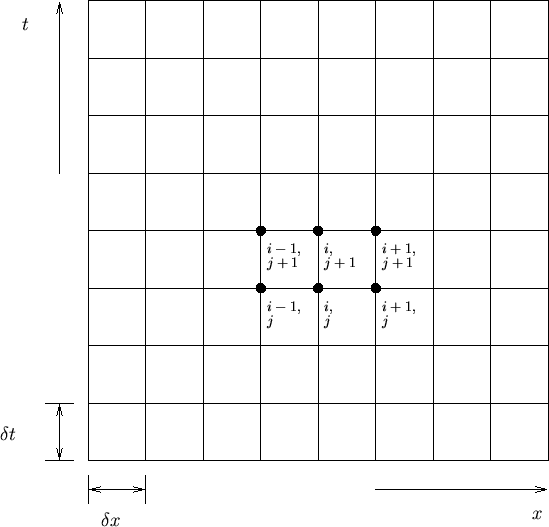
\includegraphics[scale=.45]{imagens/ilustracoes/discretizationFDM.png}
                    \caption{Domínio discretizado \cite{discreteDomainFig}}
                    \label{fig:discreteFDM}
                \end{figure}
                na qual $\delta x$ e $\delta t$ são os tamanhos dos espaços criados nas dimensões da cama elástica, que é o nosso domínio.
                
                Como podemos ver na Figura \ref{fig:discreteFDM}, a discretização do domínio leva à criação de pontos ao longo dele. Esses pontos são indexados na imagem por $i$ (referente à variável $x$) e $j$ (referente à variável $t$). Dessa forma temos que o domínio, agora discreto, do nosso problema é dado por
                \begin{align*}
                    0 \leq  &x_i \leq a\\
                    0 \leq  &t_j \leq b
                \end{align*}.
                
            \subsection{Cálculo}
            
                Tendo sido feita a discretização do domínio do problema, devemos partir para a parte dos cálculos, a ser realizada por meio das fórmulas de diferenças finitas apropriadas. Por exemplo, caso o problema fosse avaliar a função $f''(x)$ no domínio que definimos, deveríamos aplicar uma das fórmulas (\ref{u''Reg}), (\ref{u''Prog}) ou (\ref{u''Cent}) (dependendo de onde o método esteja focado no domínio do problema) para todos os pontos $(x_i, t_j)$ discretizados. Assim, obteríamos uma malha com todos os valores da derivada para todos os pontos.